\documentclass[12pt]{article}
\usepackage{amsmath}
\usepackage{mathtools}
\usepackage{bigints}
\usepackage{parskip}
\usepackage{amssymb}
\usepackage{relsize}
\usepackage{fullpage}
% \DeclareMathSizes{12}{17.28}{9}{7} % (a)

\DeclareMathSizes{12}{17.28}{12}{12} % (a)


\usepackage{hyperref}



	\addtolength{\topmargin}{-.5in}
	\addtolength{\textheight}{1.75in}



    \newenvironment{myindentpar}[1]%
     {\begin{list}{}%
             {\setlength{\leftmargin}{#1}}%
             \item[]%
     }
     {\end{list}}

\begin{document}
\title{College Algebra: Module 11 What You Need To Know}
\date{3-28-15}
\author{}
\maketitle

\section{One-to-One and Inverse Functions (Section 5.1)}

\textbf{One-to-One} - a function $f$ is \textit{one-to-one} if every element in the range corresponds to \textbf{only one} element of the domain

\textbf{Horizontal Line Test:} - a nice, easy, graphical test to determine if a function is one-to-one. It says that a function is \textbf{one-to-one} if every horizontal line intersects a graph \textbf{at most once}


\textbf{Function That Passes the Horizontal Line Test:}

\centerline{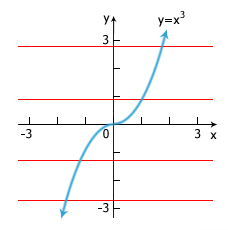
\includegraphics{PassHLT.jpg}}

\textbf{Function That Fails Horizontal Line Test:}

\centerline{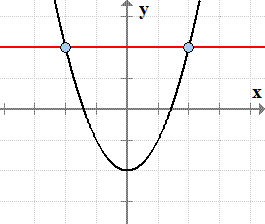
\includegraphics{FailHLT.png}}

\newpage

\textbf{Inverse Function:} - if a function $f$ is one-to-one then the \textbf{inverse function} denoted by $f^{-1}(x)$ is the function that "undoes" the original function $f$ so that
\newline

\centerline{$f^{-1}\Big(f(x)\Big) = x = f\Big(f^{-1}(x)\Big)$ }

\textbf{Properties of Inverse Function $f^{-1}(x)$ to its Original Function $f(x)$}
\begin{myindentpar}{1cm}

\begin{itemize}
\item The domain of $f^{-1}$ is the range of $f$
\item The range of $f^{-1}$ is the domain of $f$
\item Graphically, the inverse function, $f^{-1}(x)$, is the graph of the original function, $f(x)$,  reflected about the line $y=x$
\end{itemize}

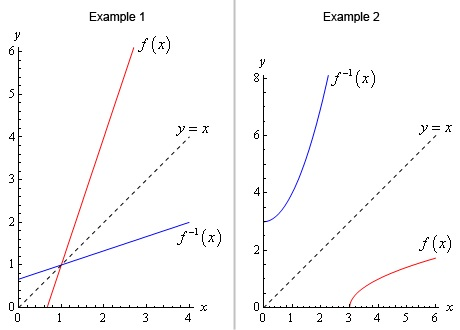
\includegraphics{InverseGraph.jpg}

\textbf{Note:} Notice how in Example 2 that the range of $f^{-1}(x)$ is the domain of $f(x)$

\end{myindentpar}

\textbf{Finding the Inverse Function:}

\begin{enumerate}
\item Set $y = f(x)$
\item Swap $x$ and $y$
\item Solve for $y$ in terms of $x$
\item The result gives the inverse function: Replace $y$ with $f^{-1}(x)$
\end{enumerate}

\newpage

\section{Exponential Functions (Section 5.2)}

\textbf{Exponential Properties}

\begin{itemize}

\item $b^{m} \cdot b^{n} = b^{m+n}$
\item $\dfrac{b^{m}}{b^{n}} = b^{m-n}$
\item $(b^{m})^{n} = b^{mn}$
\item $(a \cdot b)^{n} = a^{n} \cdot b^{n}$
\item $b^{-n} = \dfrac{1}{b^{n}}$
\item $\Big( \dfrac{b}{a} \Big)^{-n} = \Big( \dfrac{a}{b} \Big)^{n}$

\end{itemize}

\textbf{Exponential Function}
\newline

\centerline{$f(x) = b^x$ \hspace{2cm} $b\neq 1$ and $b > 0$} 

\vspace{.5cm}

\centerline{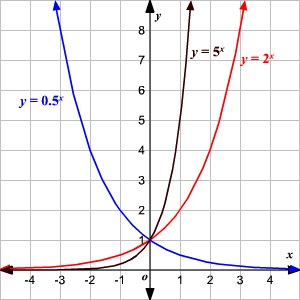
\includegraphics{ExponentialFunctionsAndGraphs.jpg}}

We say $b$ is the \textbf{base} of the exponential function.

There is a special kind of exponential function that we single out because of its significance and we call it the \textbf{Natural Exponential Function}. It is the function
\newline

\centerline{$f(x) = e^{x}$}

\textbf{Note:} $e$ is simply a number; $e \approx 2.71828...$

\textbf{Solving Exponential Equations with Common Bases}

\begin{itemize}

\item $b^{m} = b^{n} \implies m = n$ (Equal bases imply equal exponents)

\end{itemize}








































\end{document}